
    

\noindent\underline{\textbf{Kapasitor}}
\begin{enumerate}
    \begin{minipage}{0.55\textwidth}
    \item Suatu kapasitor dibentuk dari dua keping tak sejajar dengan luas keping $A$. Hitung kapasitas kapasitor ini!
    \end{minipage}
    \hfill
    \begin{minipage}{0.3\textwidth}
        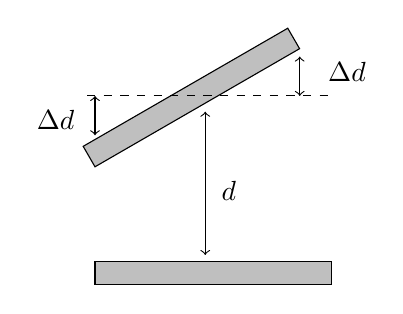
\begin{tikzpicture}
            \filldraw[fill=gray!50,rotate=30] (0,0) rectangle (3,0.3);
            \filldraw[fill=gray!50] (0,-1.2) rectangle (3,-1.5);
            \draw [dashed] (-0.1,0.9)--(3,0.9);
            \draw [<->](1.4,0.7)--(1.4,-1.12);
            \draw [<->] (0,0.4)--(0,0.9);
            \draw [<->] (2.6,0.9)--(2.6,1.4);
            \node at (1.7,-0.3) {$d$};
            \node at (-0.5,0.6){$\Delta d$};
            \node at (3.2,1.2){$\Delta d$};
        \end{tikzpicture}
    \end{minipage}
    \vskip 25pt
     \begin{minipage}{0.45\textwidth}
         \item Hitung kapasitas pengganti antara titik $P$ dan $Q$ dari rangkaian kapasitor berikut!
     \end{minipage}
     \hfill
     \begin{minipage}{0.5\textwidth}
        \begin{circuitikz}
            \draw (0,0) to [short={P},*-] (1,-0.5) to [C={$4\mu F$}] (4,-0.5);
            \draw (1,-0.5) to [short,-] (1,-0.5) to [C={$2\mu F$}] (1,-3);
            \draw (4,-0.5) to [short,-] (4,-0.5) to [C={$8\mu F$}] (4,-3);
            \draw (7,-0.5) to [short,-] (7,-0.5) to [C={$4\mu F$}] (7,-3);
            \draw (4,-0.5) to [short,-] (7,-0.5);
            \draw (1,-3) to [short,-] (4,-3);
            \draw (4,-3) to [C={$2\mu F$}] (7,-3);
            \draw (7,-3) to [short={Q},-*] (8,-3.5);
        \end{circuitikz}
     \end{minipage}

     \item Sekelompok kapasitor dihubungkan seri, lalu paralel. Kapasitas pengganti kapasitor kombinasi paralel 100 kali lebih banyak dibandingkan kombinasi seri. Hitung berapa banyak kapasitor dalam sekelompok ini!
     \vskip 10pt
    \begin{minipage}{0.55\textwidth}
    \item Suatu kapasitor keping sejajar dengan luas permukaan keping $A = 10.5 cm^{2}$ dan jarak antar keping $2d=7.12mm$, ruang antar keping diisi dengan beberapa bahan dielektrik dengan susunan sepeti gambar. Konstanta dielektrik masing-masing bahan dielektrik adalah $\kappa_1 =21, \kappa_2 =42$, dan $\kappa_3=58$
        \begin{enumerate}[a)]
            \item Tentukan kapasitansi kapasitor tersebut
            \item Tentukan muatan dan energi yang tersimpan dalam kapasitor dihubungkan dengan beda potensial $12V$
        \end{enumerate}
    \end{minipage}
    \hfill
    \begin{minipage}{0.35\textwidth}
        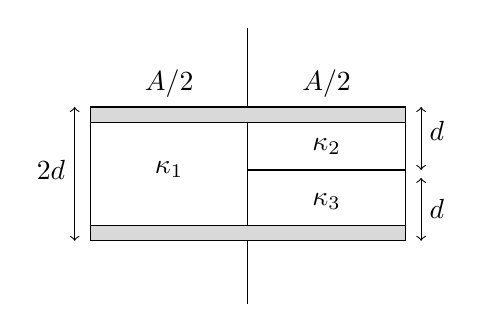
\begin{tikzpicture}
            \draw (0,0)--(0,-1);
            \filldraw [fill=gray!30] (-2,-1) rectangle (2,-1.2);
            \draw (-2,-1.2) rectangle (0,-2.5);
            \draw (0,-1.2) rectangle (2,-1.8);
            \draw (0,-1.8) rectangle (2,-2.5);
            \filldraw[fill=gray!30] (-2,-2.5) rectangle (2,-2.7);
            \draw (0,-2.7) -- (0,-3.5);
            \node at (-1,-0.7){$A/2$};
            \node at (1,-0.7){$A/2$};
            \node at (-1,-1.8){$\kappa_1$};
            \node at (1,-1.5){$\kappa_2$};
            \node at (1,-2.2){$\kappa_3$};
            \draw [<->] (-2.2,-1)--(-2.2,-2.7);
            \draw [<->] (2.2,-1)--(2.2,-1.8);
            \draw [<->] (2.2,-1.9)--(2.2,-2.7);
            \node at (-2.5,-1.8){$2d$};
            \node at (2.4,-1.3){$d$};
            \node at (2.4,-2.3){$d$};
        \end{tikzpicture}
    \end{minipage}
    
     
    \end{enumerate}